\subsection{Code similarity metrics}

We define the similarity scores on token-based, tree-based and
graph-based representations between the translated and the
reference code as the complement of string edit
distance~\cite{levenshtein}, tree edit distance~\cite{oopsla10}, and
graph edit distance~\cite{sanfeliu}, respectively.

\textbf{String similarity (STS)} is the metric to compare the
similarity of source code that is represented as a sequence of
tokens. The similarity between the translated result $T$ and its
reference code $R$ is computed as:
$$STS(R, T) = 1 - \frac{SED(S_R, S_T)}{max\left(length(S_R), length(S_T)\right)}$$
where $SED(S_R, S_T)$ is the string edit distance between the
reference sequence $S_R$ and the translated sequence $S_T$. $SED$
measures efforts that a user must edit in term of the tokens that need
to be deleted/added to transform the resulting code into the correct one;
$length(t)$ refers to the length of the sequence~$t$.

%For example, $EditDistance\left(s_R, s_T\right)$ between translated code and
%reference code in Figure~\ref{fig:issueexample2} is 4 (two deletions,
%two additions). Then, it is normalized as 0.952. Note that the closer
%the score to 1, the more similar the pair in term of lexical~tokens.

%Abstract syntax tree (AST) is the most widely-used representation in
%representing the syntactic structures in source code. Therefore,
%computing the difference of two ASTs is considered as evaluating
%syntactic difference.  In our study, we apply this idea in measuring
%the difference between the syntactic structures of reference code and
%translated code. Given a pair of methods in C\# which are need to be
%syntactically compared, we used Roslyn~\cite{roslyn} to parse them into
%ASTs. Then, we compute the tree edit distance between two trees using
%the algorithm Treed~\cite{oopsla10}. Specifically, the tree edit
%distance is calculated by number of operations ({\em add}, {\em
%delete}, {\em replace}, and {\em move}) to make them identical.

\textbf{Tree similarity (TRS)} is the metric used to measure
the similarity between two ASTs representing for the translated code $T$
and the reference code $R$:
$$TRS(R, T) = 1 -\frac{TED(AST_R, AST_T)}{size(AST_R) + size(AST_T)}$$ where $TED(AST_R, AST_T)$ is the edit
distance between the ASTs of the reference code $AST_R$ and the
translated code $AST_T$. $TED$ is calculated by the minimum number of
editing operations on AST nodes ({\em add}, {\em delete}, {\em
  replace}, and {\em move}) to sequentially make $AST_R$ and $AST_T$
identical \cite{oopsla10}; and $size(t)$ returns the number of
nodes in the AST $t$.
%
%For any two trees, there will always exist at least one editing (such
%as the one that deletes all the nodes of the first tree and inserts all
%the nodes of the second). Therefore, there will always exist at least
%one TREED value and the higher value it is, the more similar those
%trees are.
%
%\begin{figure}[h]
%	\caption{Tree Editing Example: In the label of each node, its type is in capital font and its val (if exists) is in normal font}
%	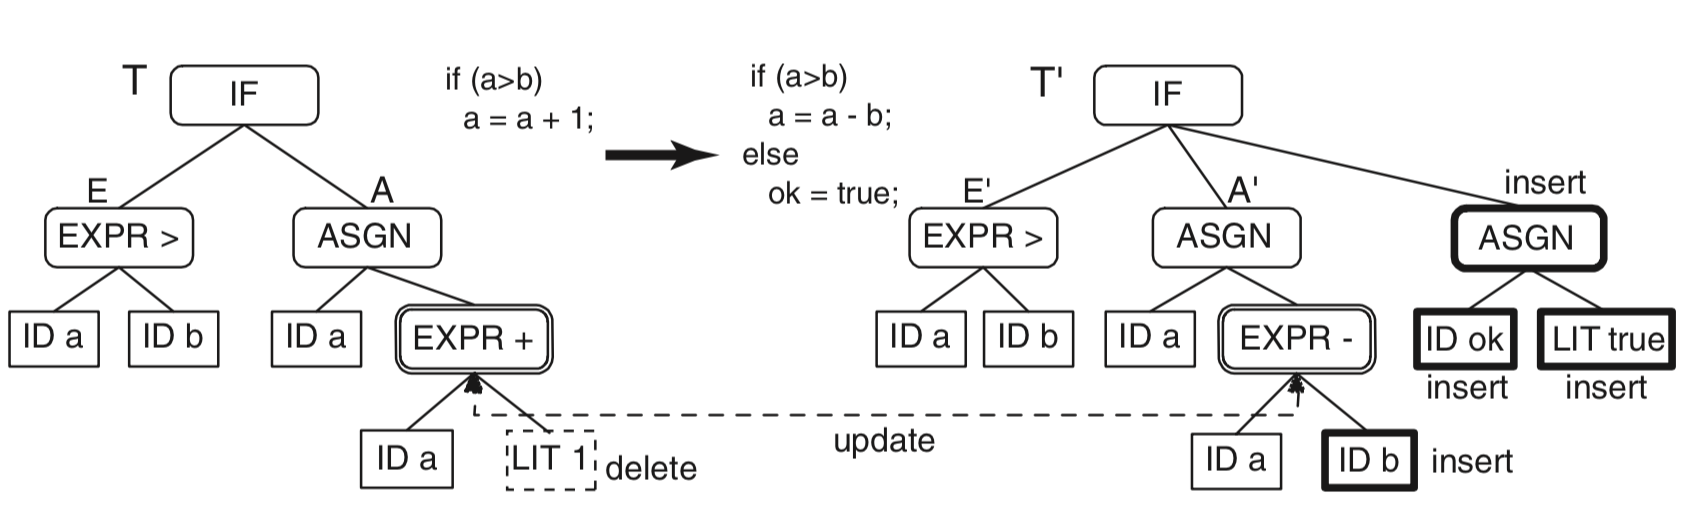
\includegraphics[scale=0.3]{img/treed.png}
%	\centering
%	\label{fig:treed}
%\end{figure}
%
%In the example in Figure \ref{fig:treed}, an \textit{if} statement was
%edited by modifying the \textit{if} branch and adding an \textit{else}
%branch. The two ASTs represent the two versions of a method. An edit
%consists of one \textit{Delete} (dotted line box), one \textit{Update}
%(double-line box), and four \textit{Insert} operations (bold
%boxes). Other nodes (single- line boxes) are either unchanged or
%moved. Based on the formula of TREED, the result in this case is:
%$TREED = 1 - \frac{1 + 1 + 4}{16}=0.625$.

%\subsubsection{\textbf{Graph Vector Edit Distance (GVED)}}
%
%Graph-based approaches in representing program semantics have become
%popular. Among those approaches, PDGs are one of the most popular.  To
%capture the graph structures in PDGs, we choose Exas~\cite{fase09}.
%Exas is an efficient structural characteristic feature extraction
%approach that approximates and captures the structure within the
%fragments of artifacts~\cite{fase09}.  In our study, we use Exas as a
%mean of computing the difference between two PDGs. Given a pair of
%method in C\# which are need to be compared, their respective
%(PDGs) are built.
%% with some additional nodes from GROUM~\cite{fse09}.
%Exas vectors will be computed on those graphs. In Exas, the
%characteristic features are extracted from the patterns of elements of
%the graphs. The code fragments are characterized by their counting
%vectors of those features. The difference between two vectors reflects
%the difference of two graphs.

%TODO cite Sanfeliu, Alberto; Fu, King-Sun (1983). "A distance measure between attributed relational graphs for pattern recognition"
In this work, we define \textbf{graph similarity (GRS)} between the
translated result $T$ and the reference code $R$ represented as PDGs
by using graph edit distance~\cite{sanfeliu}. That is:
$$GRS(R, T) = 1-\frac{GED(PDG_R, PDG_T)}{size(PDG_R)+ size(PDG_T)}$$ where $GED(PDG_R, PDG_T)$ is the edit distance
between the PDG of the reference code $PDG_R$ and the PDG of the
translated code $PDG_T$; $size(g)$ is the sum of the number of
vertexes and edges of the graph $g$. Specifically, $GED(PDG_R, PDG_T)$
is computed as the minimum number of graph edit operations to
transform one graph to another. The feasible graph edit operations on
vertexes and edges include {\em insert}, {\em delete}, and {\em
  substitute}.  However, computing the graph edit distance between two
graphs is NP-hard.  In this work, we use Exas~\cite{fase09}, a highly
precise approximate technique to compute $GED$.


%Therefore, distance of these counting vectors is considered the way to measure the sematic between code fragments.

%Figure~\ref{fig:PDGs} shows the PDGs of the code fragments 1 and
%2. These graphs are analysed by Exas, which focuses on two kinds of
%patterns of structural information of the graph, called $\left(p,q\right)$-node
%and $n$-path as can be seen in Table~\ref{tab:feature1} and
%Table~\ref{tab:feature2}.
%
%An efficient way to express the property ``having the same or similar
%features'' is to use vectors. The characteristic vector of a fragment
%is the occurrence-count vector of its features. That is, each position
%in the vector is indexed for a feature and the value at that position
%is the number of occurrences of that feature in the
%fragment. Table~\ref{tab:featureIndex} shows the indexes of the
%features, which are global across all vectors. Based on the occurrence
%counts, the vectors for code fragment 1 and~2 are
%$V_1$(1,1,1,1,1,0,1,0...) and $V_2$(1,1,0,1,1,1,1,1...),
%respectively. Two fragments having the same feature sets and
%occurrence counts will have the same vectors. The
%vector similarity can be measured by a chosen vector distance such as
%1-norm distance.
%
%We introduce the formula for normalizing the result of vector edit
%distance which is used in our experiments. The normalized
%value is described as
%\[GVED \left( V_1, V_2 \right) = 1 - \sum_{i=1}^{n} \frac{ \mid XV1_i - XV2_i \mid}{XV1_i + XV2_i}\]
%where $n$ denotes the number of vector scalar, $V_1$ denotes the
%counting vector of the first graph, $V_2$ denotes the counting vector
%of the second graph; $XV1_i$ denotes the value of the ($i-th$) scalar
%of $V_1$; and $XV2_i$ denotes the value of the ($i-th$) scalar of
%$V_2$.
%
%In this example in Figure~\ref{code1code2}, the value of GVED is
%$GVED\left(V_1, V_2\right) = 1 - \frac{8 }{20} = 0.6 $.
%
%\begin{figure}
%\begin{lstlisting}[language=JAVA]
%	Code 1:
%	void foo(int i) {
%		int j;
%		if (i < 2) {
%			j = 1;
%		} else {
%			j = 2;
%		}
%	}
%
%	Code 2:
%	void foo(int i) {
%		int j;
%		if (i < 2)
%			j = i;	
%		j = 2;
%	}
%\end{lstlisting}
%\caption{Example of two code fragments}
%\label{code1code2}
%\end{figure}
%
%\begin{figure}[t]
%	\caption{An example: two PDGs represent code fragments 1 and 2}
%	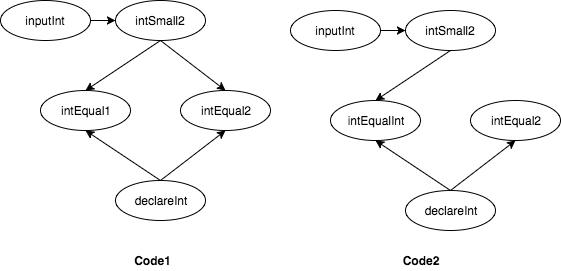
\includegraphics[scale=0.4]{img/Diagram_PDG.png}
%	\centering
%	\label{fig:PDGs}
%\end{figure}
%
%% Table generated by Excel2LaTeX from sheet 'Sheet1'
%\begin{table}[t]
%  \centering
%  \caption{Feature Table of Code Fragment 1 in Exas}
%  \scalebox{0.65}{
%    \begin{tabular}{|l|l|l|l|l|r|}
%    \toprule
%    \textbf{Pattern} & \multicolumn{5}{c|}{\textbf{Feature of Code1}} \\
%    \midrule
%    \textit{\textbf{1-path}} & inputInt & intSmall2 & intEqual1 & intEqual2 & \multicolumn{1}{l|}{declareInt} \\
%    \midrule
%    \textit{\textbf{2-path}} & \multicolumn{1}{p{6.415em}|}{inputInt-intSmall2} & \multicolumn{1}{p{5.915em}|}{intSmall2-intEqual1} & \multicolumn{1}{p{6em}|}{intSmall2-intEqual2} & \multicolumn{1}{p{5.75em}|}{declareInt-intEqual1} & \multicolumn{1}{p{5em}|}{declareInt-intEqual2} \\
%    \midrule
%    \textit{\textbf{3-path}} & \multicolumn{1}{p{6.415em}|}{intputInt-intSmall2-intEqual1} & \multicolumn{1}{p{5.915em}|}{intputInt-intSmall2-intEqual2} &       &       &  \\
%    \midrule
%    \textit{\textbf{(p,q)-node}} & inputInt-0-1 & intSmall2-1-2 & intEqual1-2-0 & intEqual2-1-2 &  \\
%    \bottomrule
%    \end{tabular}%
%	}
%  \label{tab:feature1}%
%\end{table}%
%
%% Table generated by Excel2LaTeX from sheet 'Sheet1'
%\begin{table}[t]
%  \centering
%	\caption{Feature Table of Code Fragment 2 in Exas}
%	\scalebox{0.65}{
%	    \begin{tabular}{|l|l|l|l|l|r|}
%    \toprule
%    \textbf{Pattern} & \multicolumn{5}{c|}{\textbf{Feature of Code2}} \\
%    \midrule
%    \textit{\textbf{1-path}} & inputInt & intSmall2 & intEqualInt & intEqual2 & \multicolumn{1}{l|}{declareInt} \\
%    \midrule
%    \textit{\textbf{2-path}} & \multicolumn{1}{p{6.415em}|}{inputInt-intSmall2} & \multicolumn{1}{p{5.915em}|}{intSmall2-intEqualInt} & \multicolumn{1}{p{6em}|}{declareInt-intEqual1} & \multicolumn{1}{p{5.75em}|}{declareInt-intEqual2} &  \\
%    \midrule
%    \textit{\textbf{3-path}} & \multicolumn{1}{p{6.415em}|}{intputInt-intSmall2-intEqualInt} &       &       &       &  \\
%    \midrule
%    \textit{\textbf{(p,q)-node}} & inputInt-0-1 & intSmall2-1-1 & intEqualInt-2-0 & intEqual2-1-0 &  \\
%    \bottomrule
%    \end{tabular}%
%	}
%  \label{tab:feature2}%
%\end{table}%
%
%% Table generated by Excel2LaTeX from sheet 'Sheet1'
%\begin{table}[htbp]
%	\centering
%	\caption{Feature Indexing}
%	\scalebox{0.75}{
%	\begin{tabular}{|cccc|}
%		\toprule
%		\multicolumn{1}{|l|}{\textbf{Feature}} & \multicolumn{1}{l|}{\textbf{Index}} & \multicolumn{1}{l|}{\textbf{Counted in Code1}} & \multicolumn{1}{l|}{\textbf{Counted in Code2}} \\
%		\midrule
%		\multicolumn{1}{|l|}{inputInt} & \multicolumn{1}{r|}{1} & \multicolumn{1}{r|}{1} & \multicolumn{1}{r|}{1} \\
%		\midrule
%		\multicolumn{1}{|l|}{intSmall2} & \multicolumn{1}{r|}{2} & \multicolumn{1}{r|}{1} & \multicolumn{1}{r|}{1} \\
%		\midrule
%		\multicolumn{1}{|l|}{intEqual1} & \multicolumn{1}{r|}{3} & \multicolumn{1}{r|}{1} & \multicolumn{1}{r|}{0} \\
%		\midrule
%		\multicolumn{1}{|l|}{intEqual2} & \multicolumn{1}{r|}{4} & \multicolumn{1}{r|}{1} & \multicolumn{1}{r|}{1} \\
%		\midrule
%		\multicolumn{1}{|l|}{declareInt} & \multicolumn{1}{r|}{5} & \multicolumn{1}{r|}{1} & \multicolumn{1}{r|}{1} \\
%		\midrule
%		\multicolumn{1}{|l|}{intEqualInt} & \multicolumn{1}{r|}{6} & \multicolumn{1}{r|}{0} & \multicolumn{1}{r|}{1} \\
%		\midrule
%		\multicolumn{1}{|p{5.75em}|}{inputInt-intSmall2} & \multicolumn{1}{r|}{7} & \multicolumn{1}{r|}{1} & \multicolumn{1}{r|}{1} \\
%		\midrule
%		\multicolumn{1}{|l|}{intEqual2-1-0} & \multicolumn{1}{r|}{8} & \multicolumn{1}{r|}{0} & \multicolumn{1}{r|}{1} \\
%		\midrule
%		\multicolumn{4}{|c|}{To be continued} \\
%		\bottomrule
%	\end{tabular}%
%	}
%	\label{tab:featureIndex}%
%\end{table}%




